\documentclass[aspectratio=169]{beamer}

\usepackage[utf8]{inputenc}
\usetheme{Madrid}
\usecolortheme{beaver}

\usepackage{graphicx}
\graphicspath{ {./Resources/} }

\title{Project Development Plan}       % Title
\author{Austin, Joe, Matt, Kathryn}                     % Team members
\institute{SNHU/CETA}                                   % Institute
\logo{
\includegraphics[height=0.8cm]{../../AJMK_Logo}}  % Our Logo
\titlegraphic{
\includegraphics[height=2.6cm]{Stencil.png}} % Title graphic

\begin{document}

\frame{\titlepage} % Draw the title page

\section{Introduction}
\begin{frame}
    \frametitle{Problem Statement}

    \begin{columns}

    \begin{column}{0.4\textwidth}
        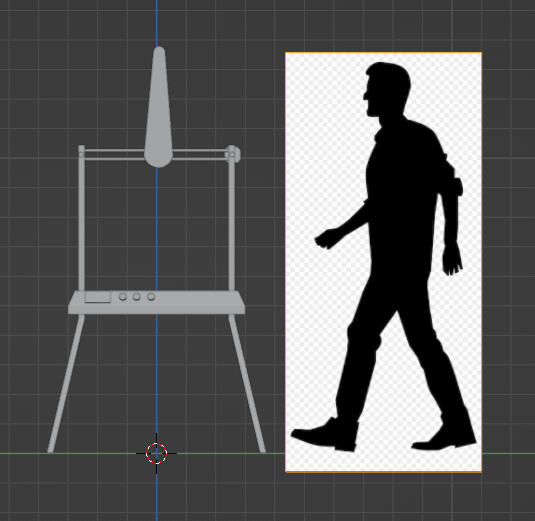
\includegraphics[height=5cm]{Scale}
    \end{column}

    \begin{column}{0.58\textwidth}
        \begin{block}{Our Goal}
        The goal is to make a PID Demonstrator that teaches the operator how to use a PID loop.
        The operator will have control to adjust each individual variable and see how each effects a
        vertical standing pendulum.
    \end{block}
    \end{column}
\end{columns}
\end{frame}

\begin{frame}
    \frametitle{Agenda}

    \begin{columns}
    \begin{column}{0.48\textwidth}
        \small{\tableofcontents}
    \end{column}

    \begin{column}{0.48\textwidth}
        \begin{center}
            
\includegraphics[height=3cm]{../../AJMK_Logo}
            
\includegraphics[height=3cm]{Stencil.png}
        \end{center}
    \end{column}
    \end{columns}
\end{frame}

\section{Research}
\begin{frame}
    \frametitle{Research}

    There are a few different approaches to the PID demonstrator system.

    \begin{columns}

    \begin{column}{0.48\textwidth}
        \begin{block}{Rotary Inverted Pendulum}
             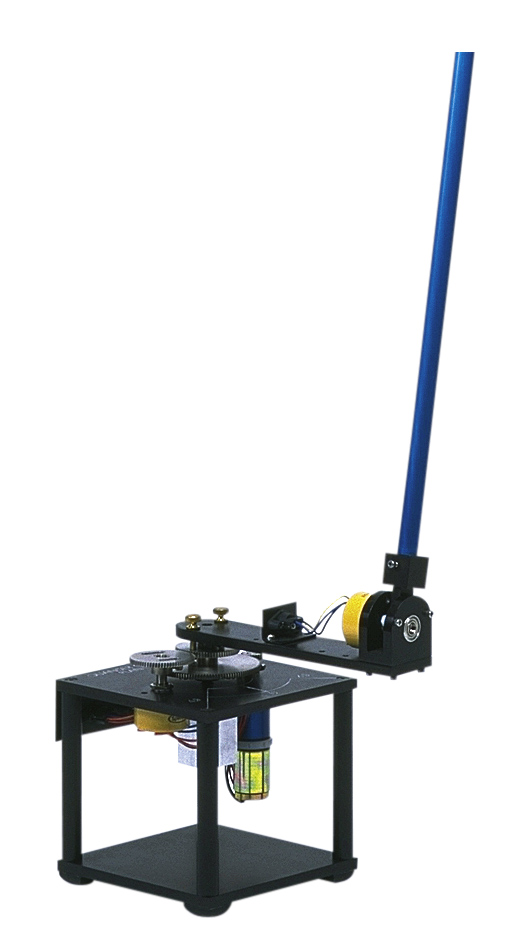
\includegraphics[height=4cm]{RotaryInvertedPendulum}
        \end{block}
        Spins around an axis to produce its motion.
    \end{column}

    \begin{column}{0.48\textwidth}
        \begin{block}{Reaction Wheel Pendulum}
                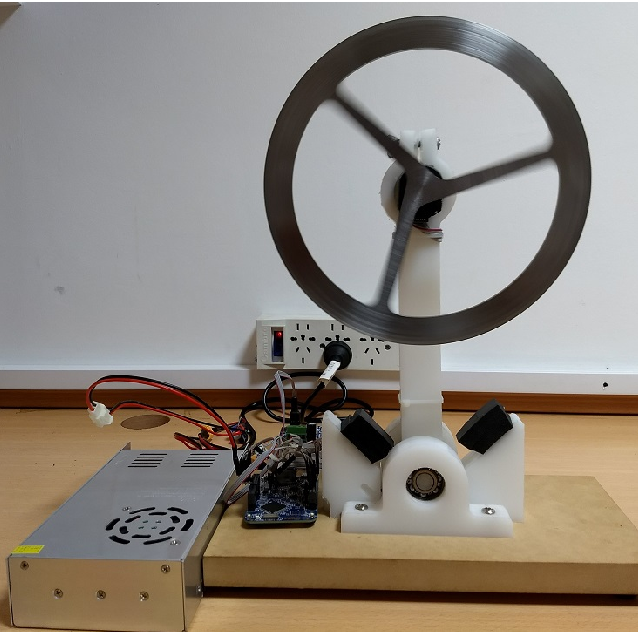
\includegraphics[height=4cm]{ReactionWheel}
        \end{block}
        Uses a reaction wheel to develop a torque against falling over.
    \end{column}
\end{columns}
\end{frame}

\section{ConOps}
\begin{frame}
    \frametitle{ConOps}

    \begin{columns}

    \begin{column}{0.34\textwidth}
        Stakeholders
        \begin{itemize}
         \item SNHU
         \item Professors
         \item Industrial Trainers
         \item Parts and manufacturers
        \end{itemize}

        Users
        \begin{itemize}
         \item Pendulum Team
         \item Educators
        \end{itemize}
    \end{column}

    \begin{column}{0.65\textwidth}
        \begin{block}{Operating Modes}
            \begin{enumerate}
            \item Off mode
            \item Idle mode
            \item Spinup mode
            \item Demo mode
            \item User PID mode
            \end{enumerate}
        \end{block}

        \begin{block}{System Description}
            \small{An inverted pendulum is a type of PID Demonstrator, where a simple PID loop
            controls and minimizes the error in a system, in this case, the error is the angle of the pendulum. A perfectly tuned PID loop will hover the pendulum.}
            \textbf{Perfectly Still}.
        \end{block}
    \end{column}
\end{columns}
\end{frame}

\begin{frame}
    \frametitle{ConOps (cont.)}

    \begin{columns}
        \begin{column}{0.48\textwidth}
            \begin{block}{Operation and Support Environment}
                \begin{itemize}
                 \item Built from COTS (common off the shelf) parts
                 \item Designed to be serviced
                 \item Constant Uptime
                 \item Low power modes
                \end{itemize}
            \end{block}
        \end{column}

        \begin{column}{0.48\textwidth}
            \begin{block}{Impact considerations}
                \begin{itemize}
                 \item Requiring physical space, either for storage or use.
                 \item Being a hazard and risking misuse.
                 \item Generating pollutants and disposal.
                \end{itemize}
            \end{block}
        \end{column}
    \end{columns}
\end{frame}


\section{Requirements}
\subsection{System Requirements}
\begin{frame}
    \frametitle{System Requirements}

    \begin{columns}
        \begin{column}{0.48\textwidth}
            \begin{block}{System Requirements}
                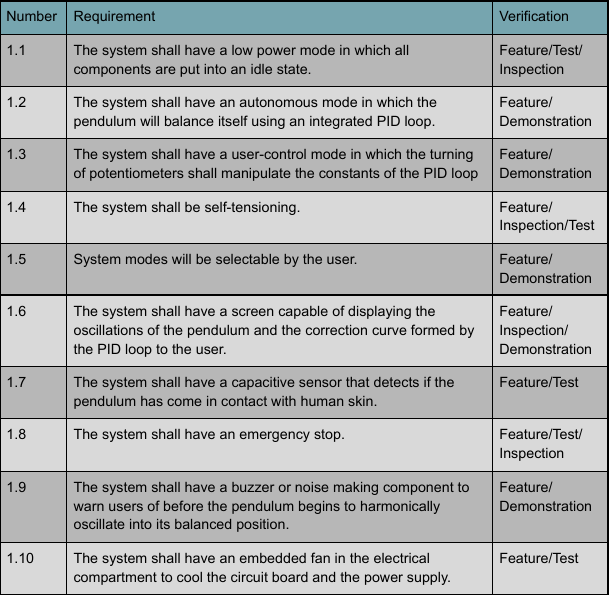
\includegraphics[height=5cm]{FunctionalRequirements}
            \end{block}
        \end{column}

        \begin{column}{0.48\textwidth}
            The functional requirements detail what will make our system, \textbf{our system}. Features
            that are required for us to actually \textbf{solve the problem} we want to solve.
            The most important features include having a \textbf{good user interface mode}, and safety
            systems like an \textbf{emergency stop and guards}.
        \end{column}
    \end{columns}
\end{frame}

\subsection{Performance Requirements}
\begin{frame}
    \frametitle{Performance Requirements}

    \begin{columns}
        \begin{column}{0.48\textwidth}
            Performance Requirements decide critical performance targets, ie, it should be so
            fast or so quiet or so efficient. The most important in our performance requirements
            are features such as \textbf{Self Starting} and function of the \textbf{Buttons}.
        \end{column}

        \begin{column}{0.48\textwidth}
            \begin{block}{Performance Assessment}
                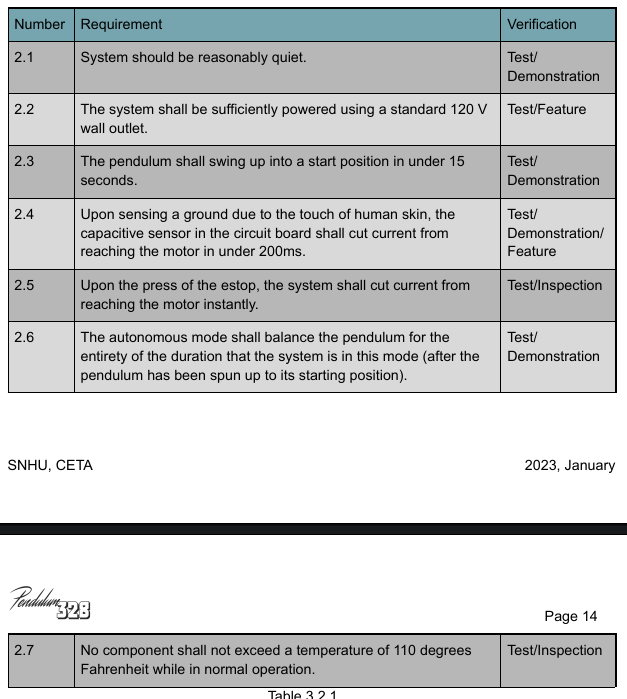
\includegraphics[height=5cm]{PerformanceRequirement}
            \end{block}
        \end{column}
    \end{columns}
\end{frame}

\subsection{Physical Requirement}
\begin{frame}
    \frametitle{Physical Requirements}

    \begin{columns}
        \begin{column}{0.48\textwidth}
            \begin{block}{Physical Requirements}
                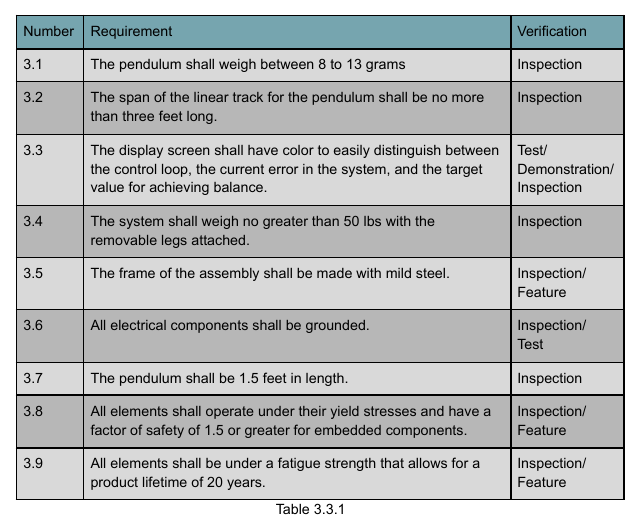
\includegraphics[height=5cm]{PhysicalRequirement}
            \end{block}
        \end{column}

        \begin{column}{0.48\textwidth}
            Physical Requirements are like the other requirements and define the physical
            attributes that define success in solving our product's problem. The most important here
            involve proper use of \textbf{Material} and physical strength requirements.
        \end{column}
    \end{columns}
\end{frame}

\subsection{Risk Assessment}
\begin{frame}
    \frametitle{Risk Assessment}

    \begin{columns}
        \begin{column}{0.48\textwidth}
            Any product or plan comes with risks but mitigation of risks can help make a safe
            and functional product, a couple of the most critical components of our risk assessment
            were safety involving \textbf{Pinch Points}, being \textbf{Struck by moving components}
            or the potential risk of electrical fire due to electronics inside.
        \end{column}

        \begin{column}{0.48\textwidth}
            \begin{block}{Risk Assessment}
                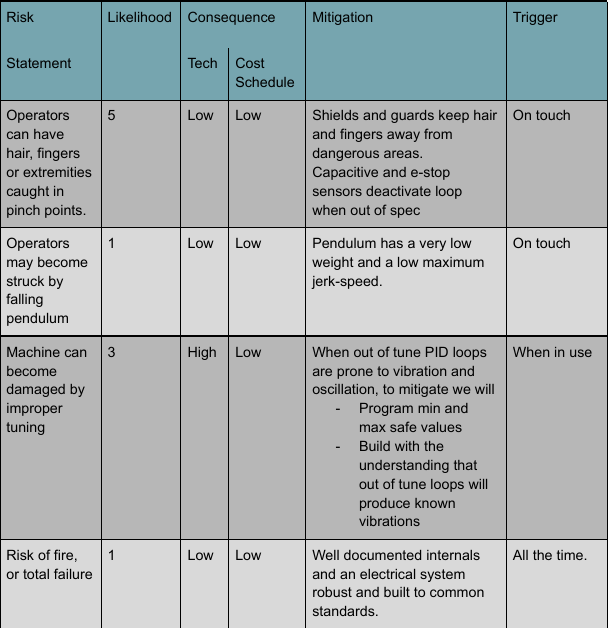
\includegraphics[height=5cm]{RiskAssesment}
            \end{block}
        \end{column}
    \end{columns}
\end{frame}

\subsection{Enviormental Requirements}
\begin{frame}
    \frametitle{Environmental Requirements}

    \begin{columns}
        \begin{column}{0.48\textwidth}
            \begin{block}{Environmental Requirements}
                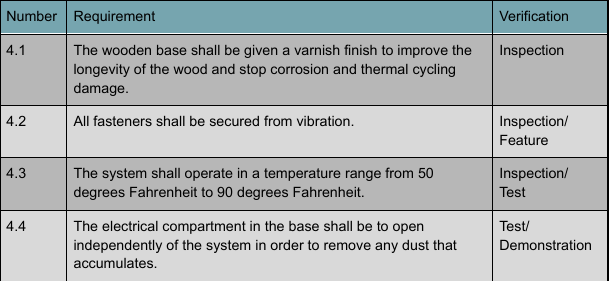
\includegraphics[width=7.3cm]{EnviromentalAndSafety}
            \end{block}
        \end{column}

        \begin{column}{0.48\textwidth}
            We know that our product will be used in some environment, if we want to design a safe
            and functional product we need to take this into account, things like \textbf{Usage schedule}
            and the quality of the air we're blowing over our electronics, mitigation of
            \textbf{dust and oils} as well.
        \end{column}
    \end{columns}
\end{frame}

\subsection{Engineering Standards}
\begin{frame}
    \frametitle{Engineering Standards}

    \begin{columns}
        \begin{column}{0.48\textwidth}
            Designing to existing engineering standards not only reduces work but makes it easier
            for another team or engineer to make modifications, repairs upgrades or ensure future
            interoperability with existing systems.
        \end{column}

        \begin{column}{0.48\textwidth}
            \begin{block}{Engineering Standards}
                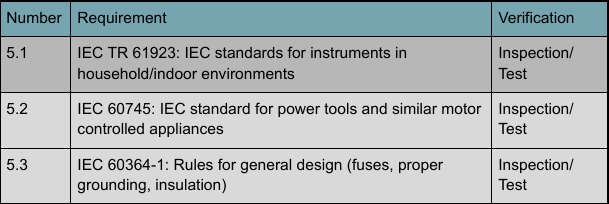
\includegraphics[width=7.3cm]{EngineeringStandards}
            \end{block}
        \end{column}
    \end{columns}
\end{frame}

\section{Design Concepts}
\begin{frame}
    \frametitle{Design Concepts (1)}

    \begin{columns}
        \begin{column}{0.48\textwidth}
            \begin{block}{Sketch 1}
                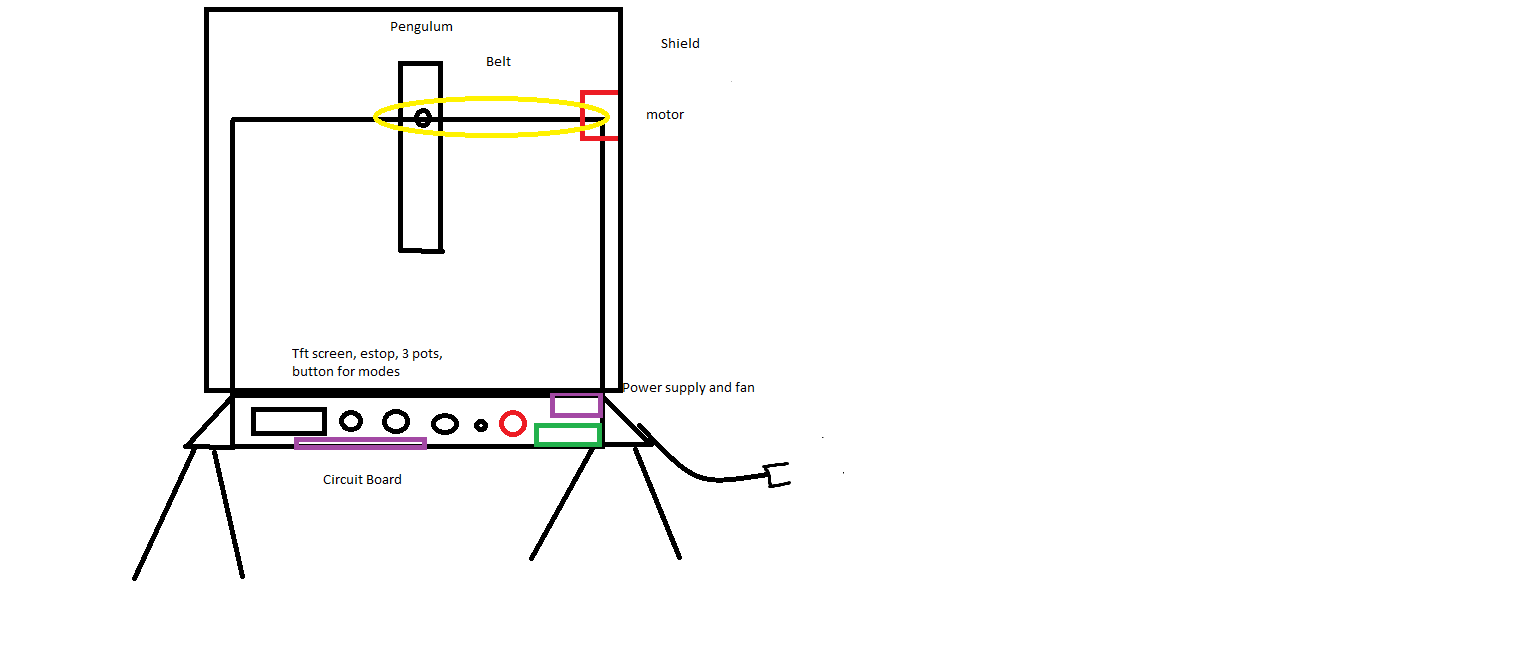
\includegraphics[height=6cm]{../../../Notes/Sketches/Basic Mock-Up Sketch.png}
            \end{block}
        \end{column}

        \begin{column}{0.48\textwidth}
            \begin{block}{Sketch 2}
                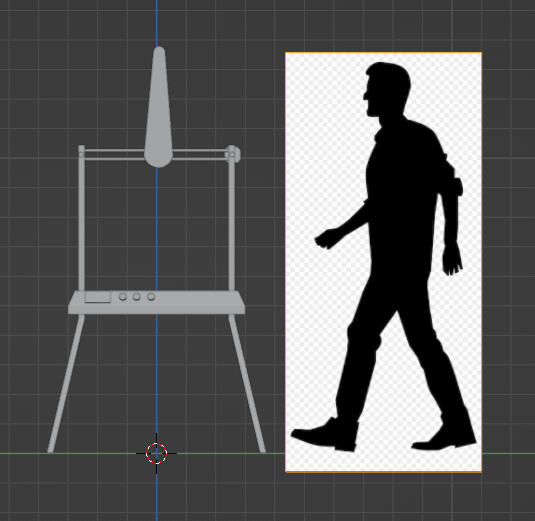
\includegraphics[height=6cm]{Scale}
            \end{block}
        \end{column}
    \end{columns}
\end{frame}

\begin{frame}
    \frametitle{Design Concepts (2)}

    \begin{columns}
        \begin{column}{0.48\textwidth}
            \begin{block}{Sketch 3}
                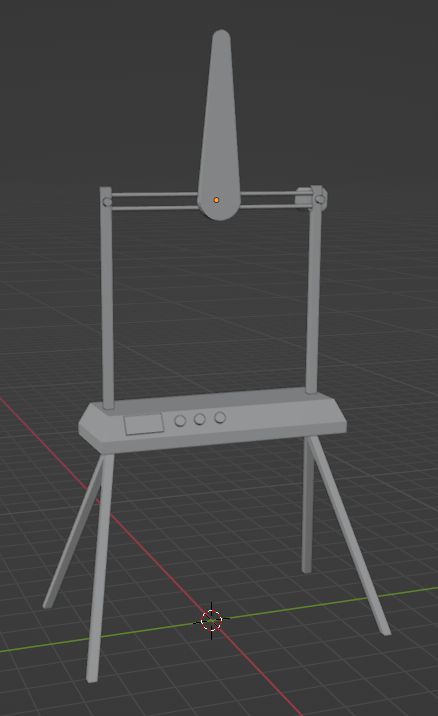
\includegraphics[height=6cm]{Full}
            \end{block}
        \end{column}

        \begin{column}{0.48\textwidth}
            \begin{block}{Sketch 4}
                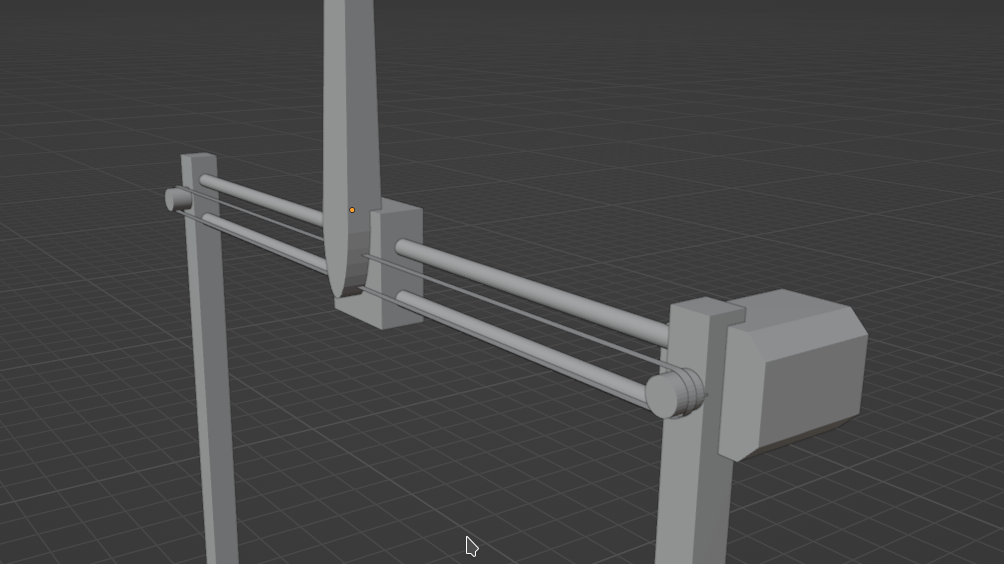
\includegraphics[width=7.3cm]{UpperAssy}
            \end{block}
        \end{column}
    \end{columns}
\end{frame}

\begin{frame}
    \frametitle{Design Concepts (3)}

    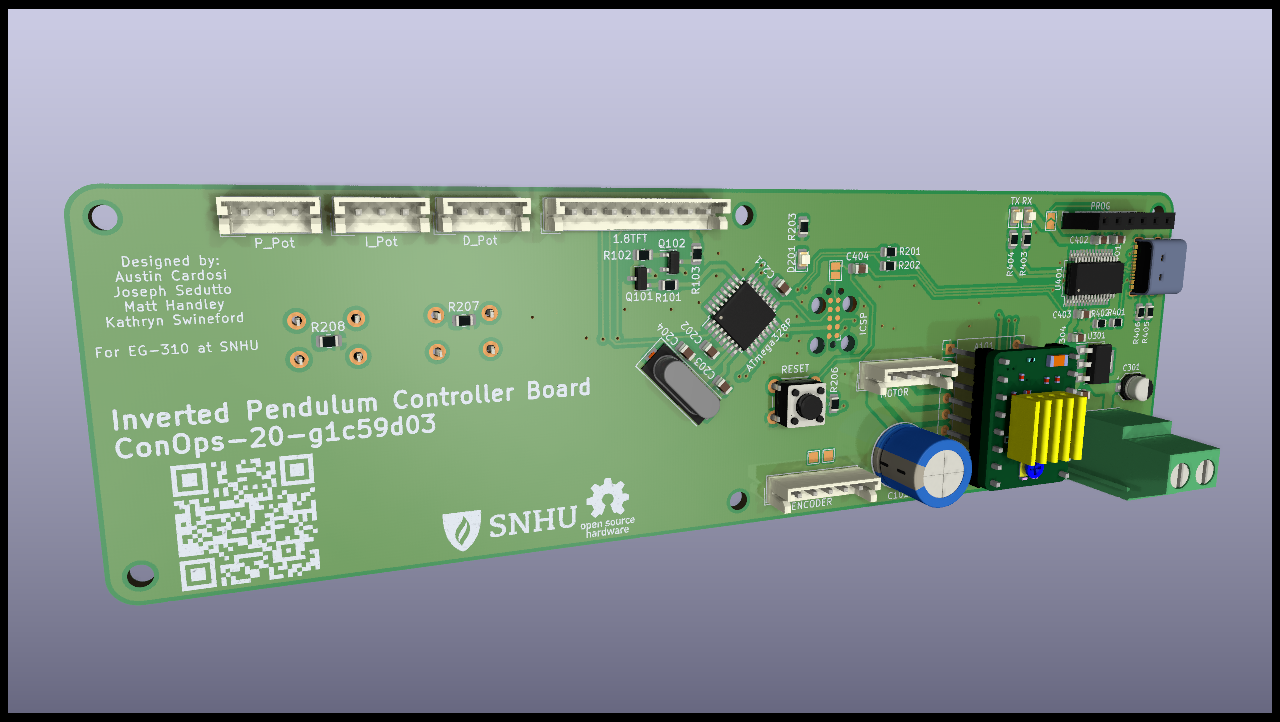
\includegraphics[width=10cm]{CircuitBoard}
\end{frame}

\begin{frame}
    \frametitle{Design Concepts (4)}

    \begin{columns}
        \begin{column}{0.48\textwidth}
            \begin{block}{Sketch 5}
                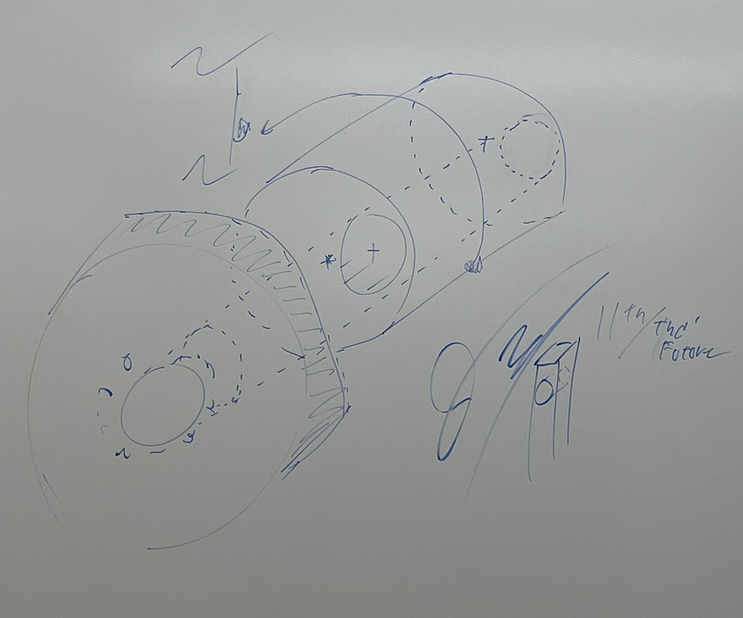
\includegraphics[height=6cm]{Tension}
            \end{block}
        \end{column}

        \begin{column}{0.32\textwidth}
            \begin{block}{Sketch 6}
                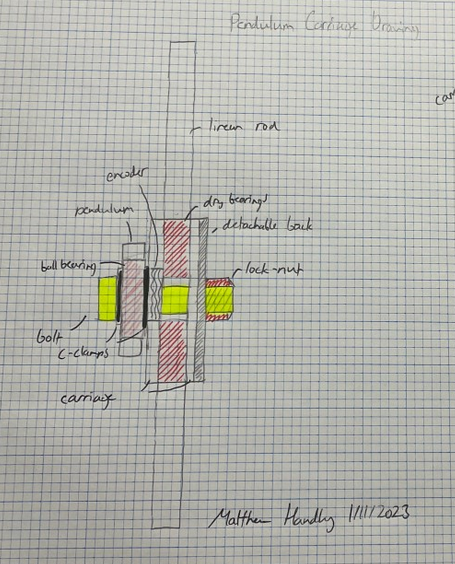
\includegraphics[height=6cm]{Carriage}
            \end{block}
        \end{column}
    \end{columns}
\end{frame}

\begin{frame}
    \frametitle{Task Plan}

    With both ProjectLibre (An open source program)

    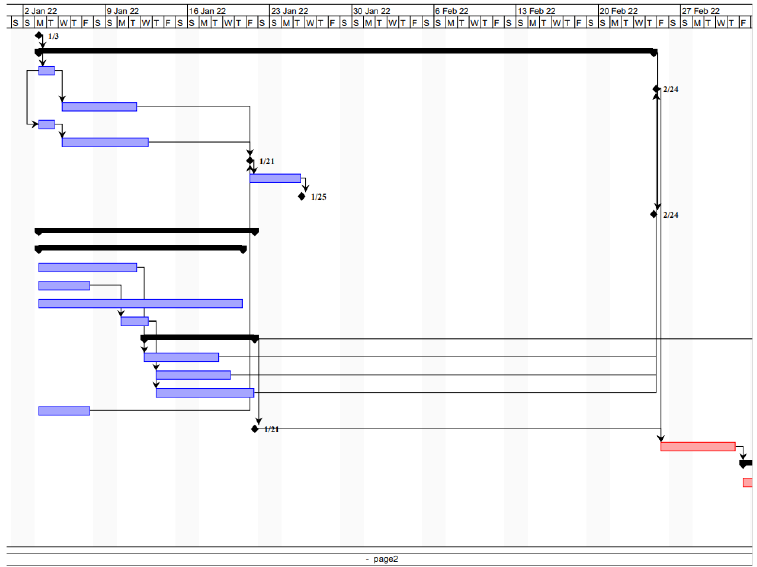
\includegraphics[height=3cm]{ProjectLibre}

    and github task management, we plan and manage our team's productivity.

    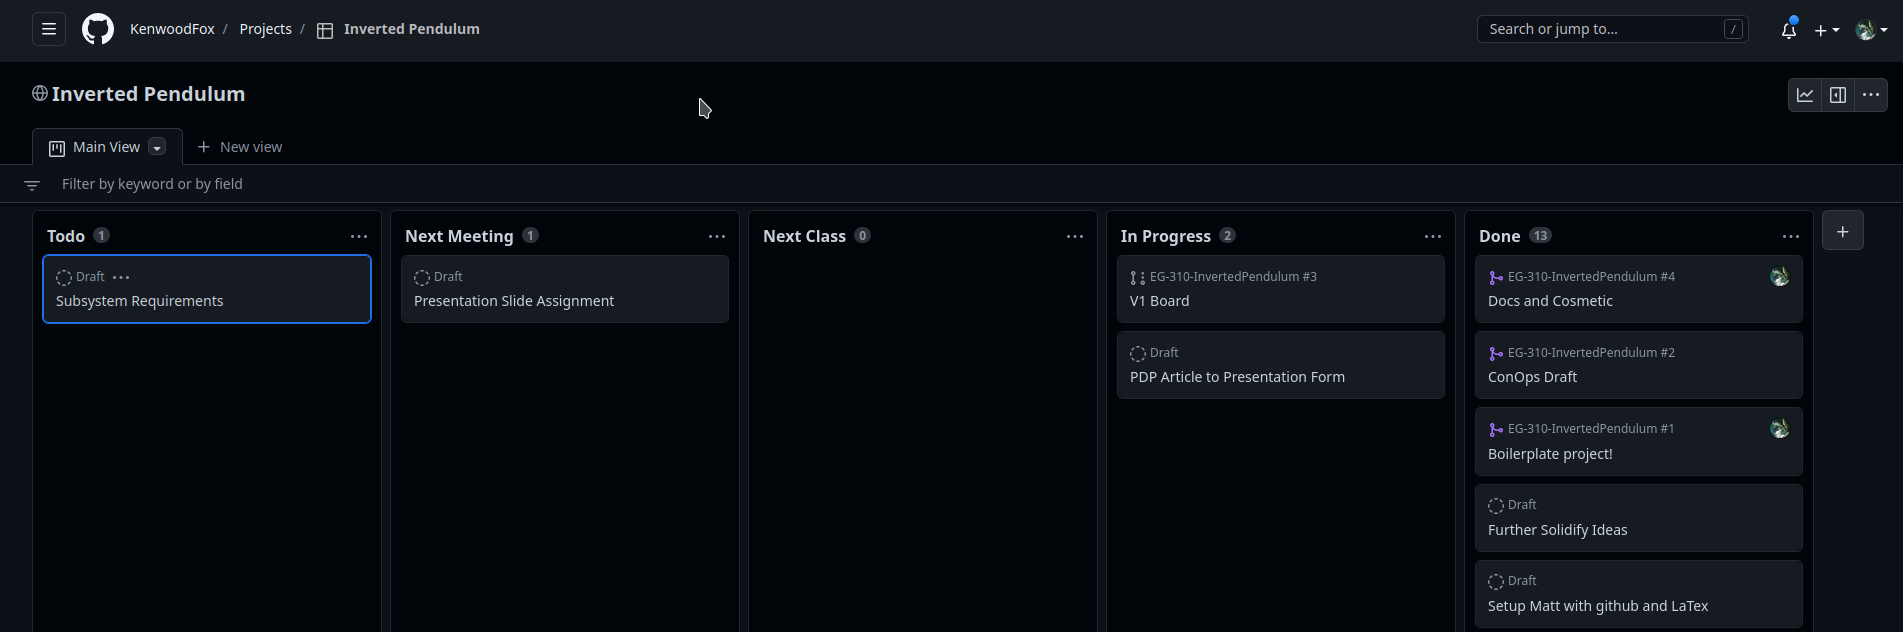
\includegraphics[width=10cm]{ProjectPlan}
\end{frame}

\section{Budget}
\begin{frame}
    \frametitle{Budget}

    \begin{columns}
        \begin{column}{0.70\textwidth}
            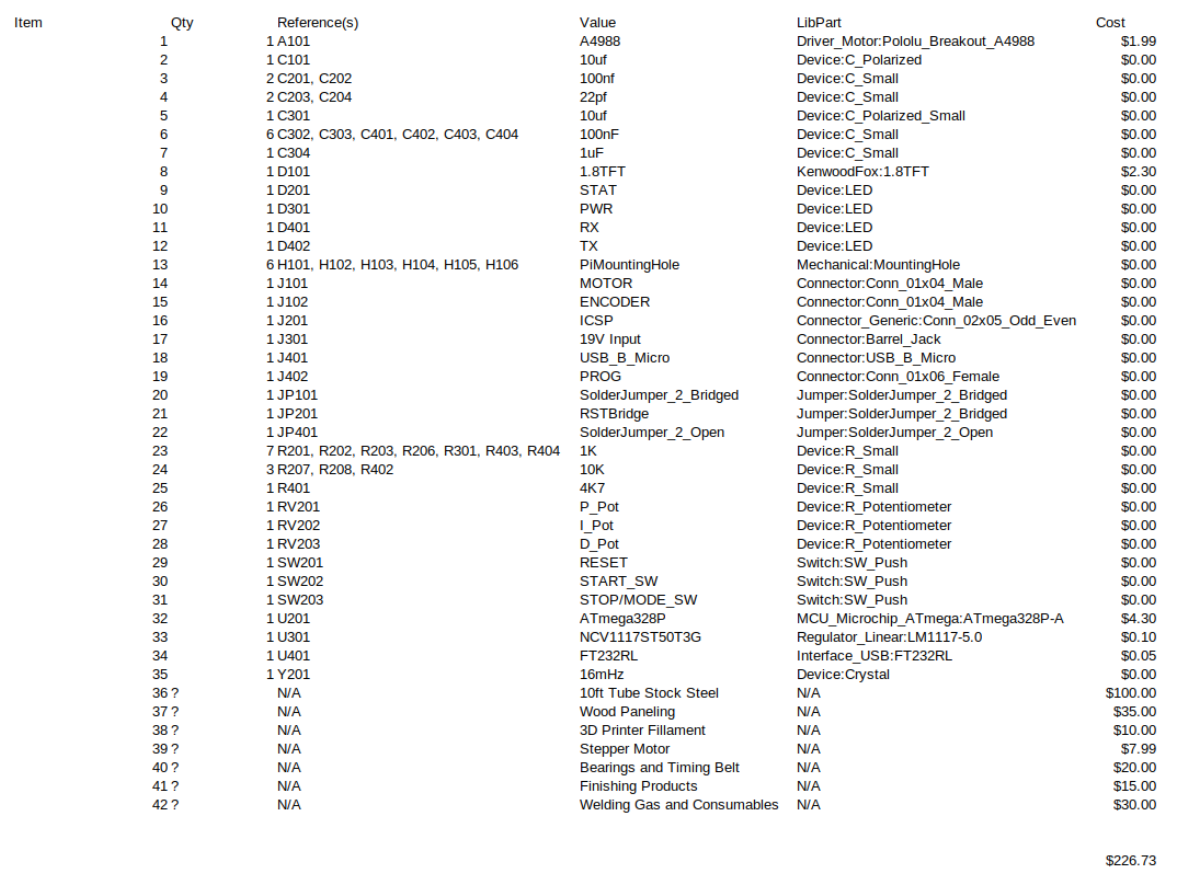
\includegraphics[height=7cm]{BOMTable}
        \end{column}

        \begin{column}{0.30\textwidth}
            We project to complete our project underbudget! With a low upfront development cost.
            We currently project spending \$250 to \$300 for our prototype.
        \end{column}
    \end{columns}
\end{frame}

\section{Diagrams}
\subsection{Block Diagrams}
\begin{frame}
    \frametitle{Block Diagram}

    \begin{columns}
        \begin{column}{0.70\textwidth}
            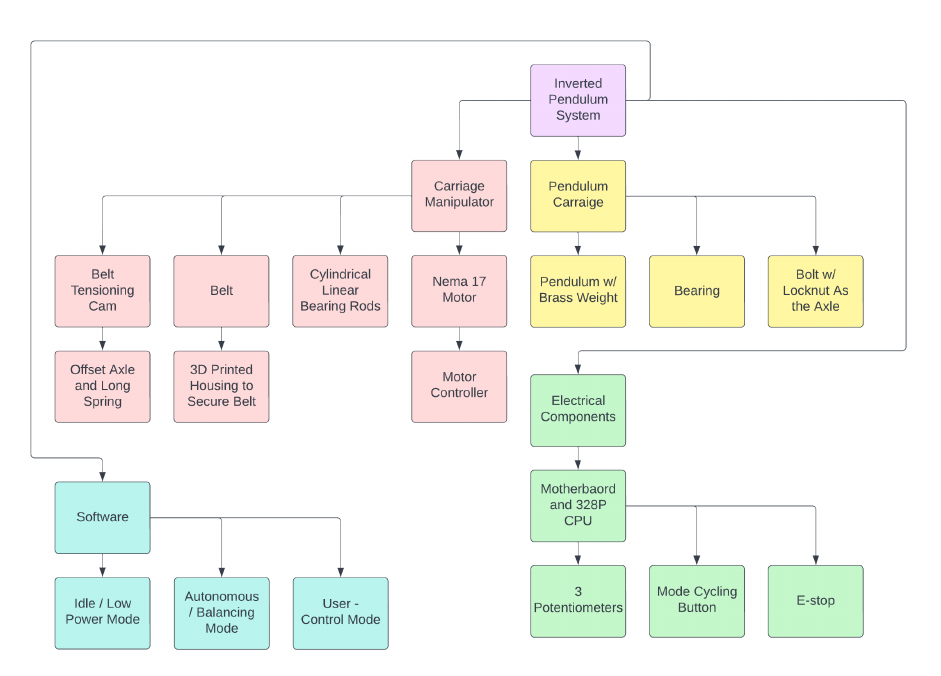
\includegraphics[height=7cm]{BlockDiagram}
        \end{column}

        \begin{column}{0.30\textwidth}
            \begin{block}{Block Diagram}
                The block diagram details the electrical, mechanical and software components.
                And their relationship to each other.
            \end{block}
        \end{column}
    \end{columns}
\end{frame}

\subsection{Operations}
\begin{frame}
    \frametitle{Operations}

    \begin{columns}
        \begin{column}{0.30\textwidth}
            \begin{block}{Operations}
                The Operations diagram details the physical and general controls.
            \end{block}
        \end{column}

        \begin{column}{0.70\textwidth}
            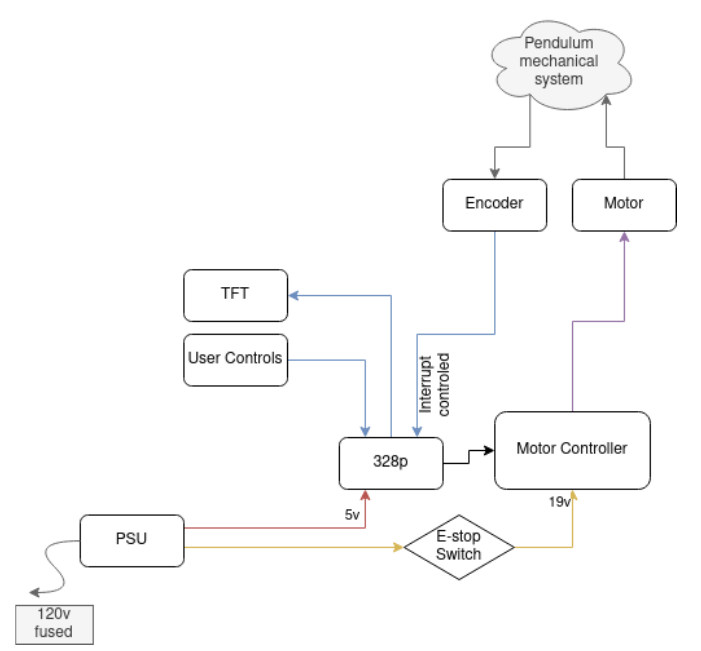
\includegraphics[height=7cm]{Operations}
        \end{column}
    \end{columns}
\end{frame}

\subsection{Software}
\begin{frame}
    \frametitle{Software Flowchart}

    \begin{columns}
        \begin{column}{0.72\textwidth}
            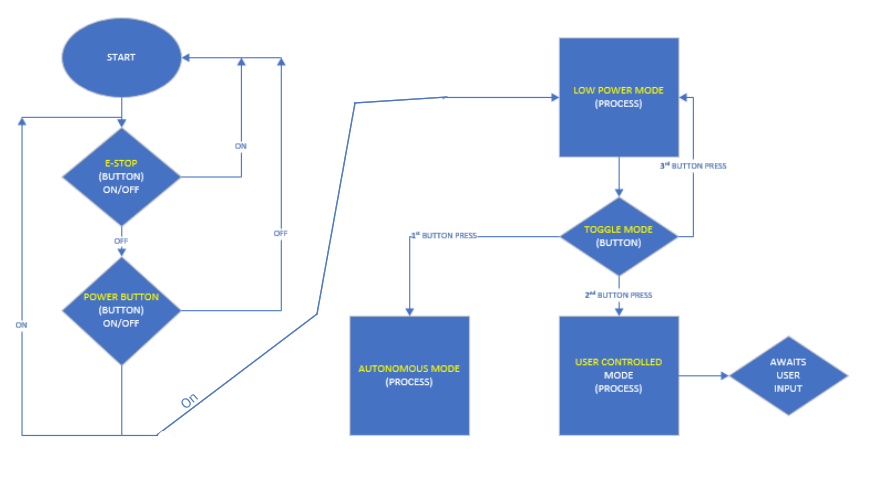
\includegraphics[width=11cm]{SoftwareFlowchart}
        \end{column}

        \begin{column}{0.28\textwidth}
            \begin{block}{Software Flowchart}
                The software flowchart is an overview of all the software functions of our
                proposed product.
            \end{block}
        \end{column}
    \end{columns}
\end{frame}

\section{End}
\begin{frame}
    \frametitle{End}

    \begin{block}{}
        \begin{center}
            \Huge Questions and Comments?
        \end{center}
    \end{block}

    \begin{center}
        Find the source code for this document, and the rest of our designs, firmware, hardware
        and notes on GitHub!

        
\includegraphics[height=2cm]{github_qr}
    \end{center}
\end{frame}

\section{Appendices}
\begin{frame}
    \frametitle{References}

    \includegraphics[height=4cm]{references}
\end{frame}

\begin{frame}
    \frametitle{Complete Timeline}

    \includegraphics[width=15cm]{project}
\end{frame}

\begin{frame}
    \frametitle{Calculations}

    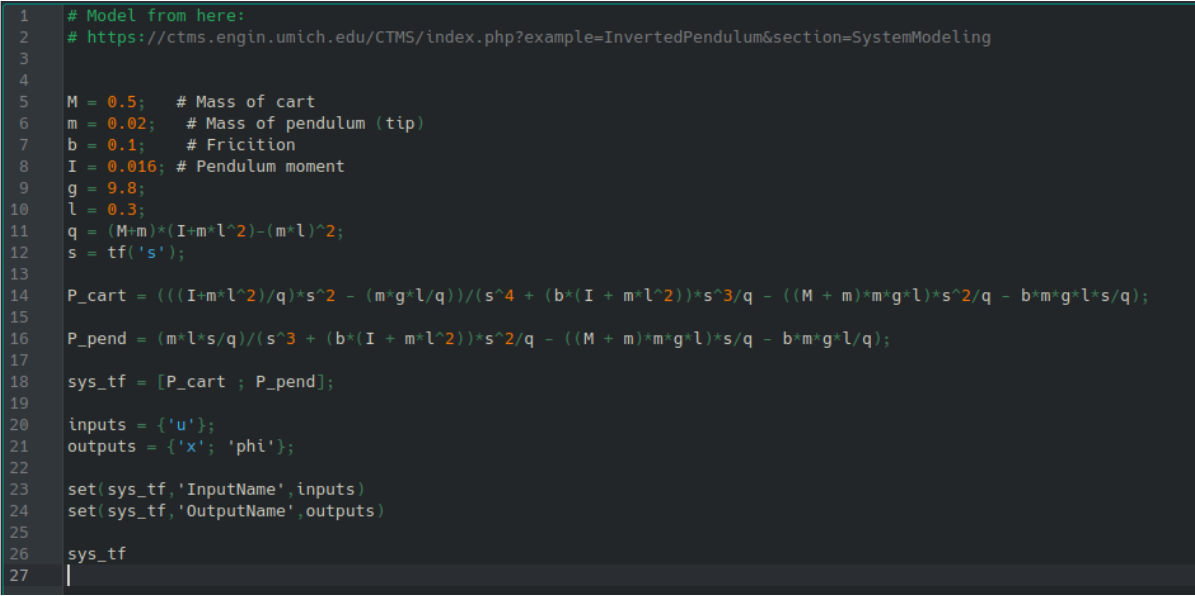
\includegraphics[height=6.5cm]{Calculations}

    Octave math model.
\end{frame}


\end{document}
